\chapter{Experiments}

This chapter \color{red} A finir \color{black}

\section{Experimental set-up configuration}

\subsection{DWM1000}

One of the feature of the DWM1000 is to store the \gls{cir} received if required. To perform such an action, the documentation provided by Decawave \cite{usermanual} was used in order to determine which bits were to be activated. It appears that several bits needed to be set in specific configuration, all in the \texttt{0x36} : \gls{pmsc} register, sub-register \texttt{0x00} which is a 32 bits control register. The control register is shown in Fig. \ref{fig:control_reg}.
\vspace{2mm}

\begin{itemize}
\item The bits 3,2 :  \text{\gls{rxckls}}  needs to be set to \texttt{10} to allow the host system to reach the \gls{cir}.
\item The bit 6 : \text{\gls{face}} needs to be set to \texttt{1} for the host system to read the accumulator data\footnote{Where the \gls{cir} is stored.}.
\item The bit 15 : \text{\gls{amce}} needs to set to \texttt{1} for the same reason as bit 6.
\end{itemize}

\begin{figure}[H]
\centering
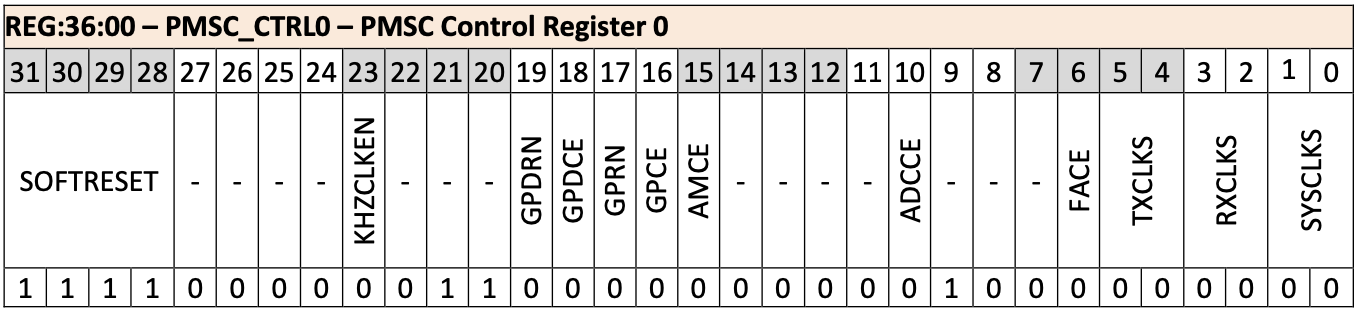
\includegraphics[width=.9\linewidth]{Images/control_ref.png}
\caption{Register \texttt{0x36} - \gls{pmsc}, sub-register \texttt{0x00}. Taken from \cite{usermanual}. \label{fig:control_reg}}
\end{figure}

When those bits are activated, we may recover the \gls{cir} from the DWM1000. Still following the manual user, it appears that the \gls{cir} is stored in the \texttt{0x25} : \text{Accumulator \gls{cir} memory register}. This register contains complex values, 16 imaginary bits and 16 real bits for each tap, 992 of them being registered when the \gls{prf} is set to 16 MHz. Each registered tap corresponds almost to a frame of 1 ns, which corresponds exactly to a sampling frequency  being twice 499.2 MHz, meaning that the whole \gls{cir} registered corresponds to almost a $\mu$s.
\vspace{2mm}

Since the algorithms developed in chapter \ref{algos} mostly work based on the direct ray and simple reflections, one may question the usefulness of extracting the whole \gls{cir} stored in the accumulator. Indeed, in a room of dimensions (15x20)m for example, in the longest first reflection that would occur, the travelled distance would be of $\sqrt(20^2 + 15^2) = 42.72m$, which corresponds to a distance time of $1.42*10^{-7}$s. Which is less than a fifth of the whole \gls{cir} stored in the accumulator.
\vspace{2mm}

In order to extract partially the \gls{cir}, the position of the peak needs to be known. This information is stored in the \texttt{0x15} : \text{\gls{rxtime}} register, in the sub-register \texttt{0x05} : \text{\gls{fpindex}} . A 16 bits long value representing the index value corresponding to leading edge of the \gls{cir} stored, only the 10 \glspl{msb} represent the integer part of this index. By taking a window around this peak, the number of bits to transmit from the DWM1000 to the PSoC can be reduced.
\vspace{2mm}

The Fig. \ref{fig:cir_long_short} shows two experimental \gls{cir} obtained, one by extracting the whole data set while the other only extracted part of it using the value stored in the \gls{fpindex} sub-register.

\begin{figure}[H]
\centering
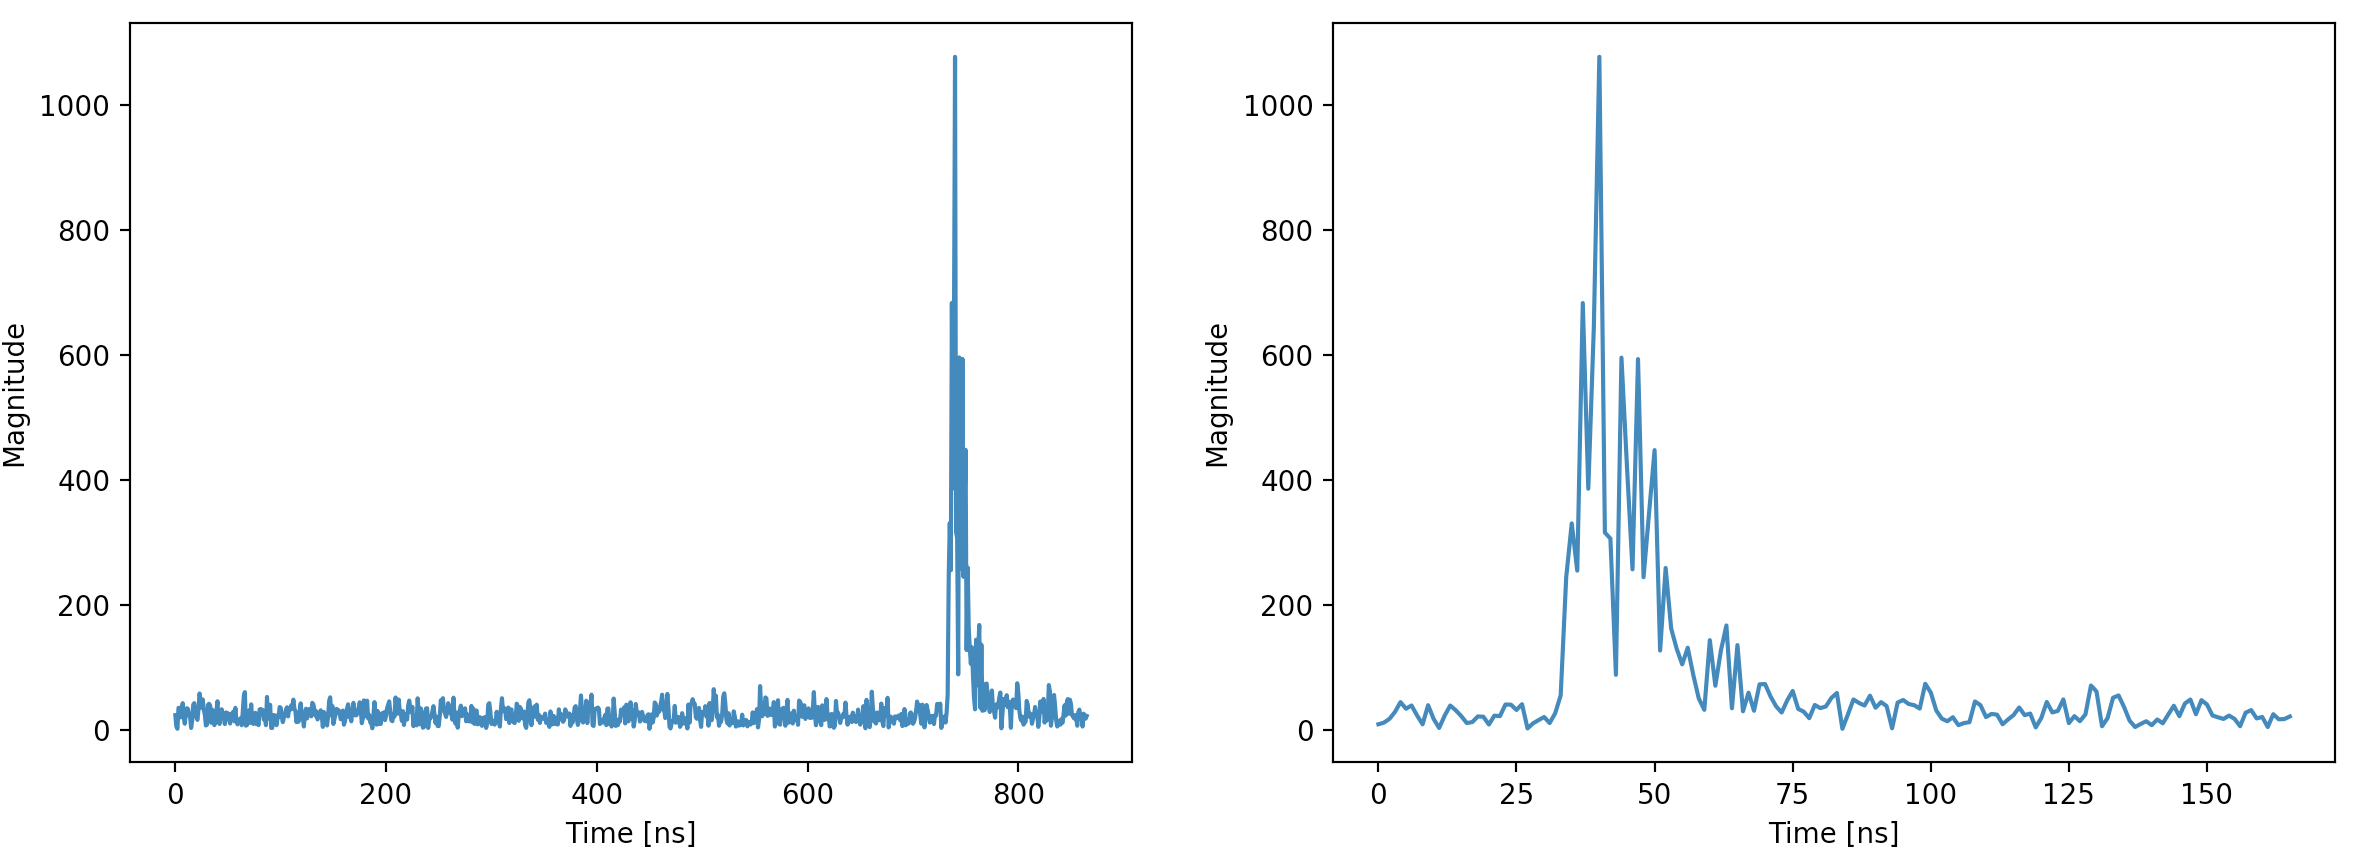
\includegraphics[width=\linewidth]{Images/extracted_cir.png}
\caption{Whole CIR extracted from the DWM1000 (Left) vs. Partial CIR extracted from the DWM1000 (Right). \label{fig:cir_long_short}}
\end{figure}

\subsection{PSoC}

The PSoC controls the DWM1000 on the tag side. Therefore, it needs to handle the \gls{cir} recuperation from register \texttt{0x25}. In order to avoid a too big modification of the interactions between the tag and the anchors, it was decided to graft this recuperation part to the existing code taking care of the \gls{sdstwr}. At the end of those exchanges, the PSoC checks that the needed bits activating the \gls{cir} recuperation are set, gets the \text{\gls{fpindex}} and partially extract the \gls{cir} around this value. In order to extract the whole \gls{cir}, 25 values before and 175 values behind were taken. This corresponds to an extracted \gls{cir} which is $\text{2*10}^\text{-7}$ \text{s} long. This choice is arbitrary and may be tuned in function of the room where the localization is performed.
\vspace{2mm}

The extraction is made through the \gls{spi} port between the DWM1000 and the PSoC, the number of bytes that needs to be extracted is 4 times the number of tap required. This number of bytes that can be transmitted through this bus at once is limited to 256 in this case. The \gls{cir} needs to be divided into several parts for one to get it all back. While extracting those data, one have to be really careful because every time the accumulator memory is accessed, the first octet output should be discarded. Indeed, it is a dummy one due to memory access. \cite{usermanual}.

\subsection{Android Application}

Since the Android Application is the master of the PSoC, it has also to be modified. Three different features were added : two activities were added and the Navigation activity was modified to achieve the \gls{cir} recuperation. 
\vspace{2mm}

The goal of the first activity is to validate the access of the application to the memory of the smartphone or an external memory in order to store data on it. In this specific case, the activity takes a string and write it into an chosen file in the memory. The final purpose being to save the extracted \gls{cir} in the memory to analyze it later. In order to access the memory, the application needs to ask some special permission to the \gls{os}. This specific android permission is called: \text{WRITE\_EXTERNAL\_STORAGE}, it will create a pop-up the first time the application will try to access the memory, asking the user if the application can have access to it.
\vspace{2mm}

The second activity is made to validate the recuperation and storage of a \gls{cir} from the DWM1000 to the memory. This activity actually imitates the 'Test USB' activity, a byte code is sent to the PSoC that triggers the recuperation function of the \gls{cir}. This \gls{cir} then needs to be transmitted to the application through the USB connection which has been already implemented. As for the PSoC, the \gls{cir} is separated into several sections to be fully transmitted through the USB connection.
\vspace{2mm}

The third feature actually combines the two new activities and the navigation one. Once again, in order to modify as less as possible the whole localization process, the \gls{cir} recuperation has been grafted. Meaning that in addition to the \gls{tof} already provided by the PSoC for each anchor, the PSoC will also provide the \gls{cir} with each anchor. This whole set of data will then be saved in a \text{'.txt'} file which is named in function of the time of execution of the program in the following format : \text{yyyy-MM-dd-hh-mm-ss.txt} i.e. \text{2020-05-30-17-05-32.txt}.
\vspace{2mm}

In order to further analyze the recuperated data, the estimated position of the tag computed by the navigation activity is saved as well. The data structure is shown in Fig. \ref{fig:saved_data}.

\begin{figure}[H]
\centering
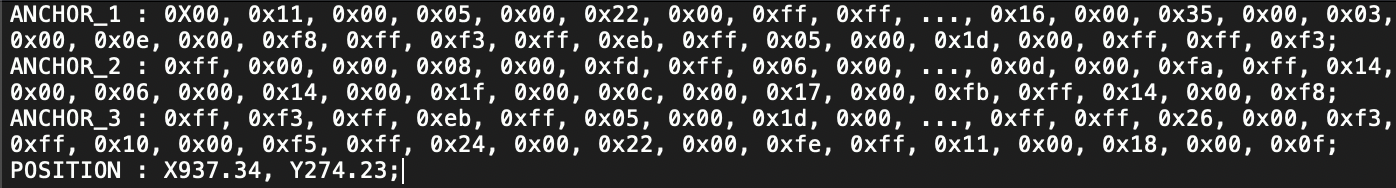
\includegraphics[width=\linewidth]{Images/saved_cir.png}
\caption{Data structure example of a measurement in navigation. \label{fig:saved_data}}
\end{figure}

For each anchor, the recuperated CIR, which is 800 octets long\footnote{800 octets long corresponds to 200 values of the \gls{cir} as 1 tap is made using 4 octets, 2 real and 2 imaginary.}, has been shortened using the \texttt{'...'} to be more visible. As we can see, each \gls{cir} is explicitly associated with an anchor and the position is stored in \text{cm} in plain text as well.

\section{Test Campaign}

The purpose behind the test campaign is to validate the simulations previously detailed, testing in a realistic case the locating algorithm using only one anchor. To reach this goal, an experiment was planned. Because of the exceptional situation linked to the COVID-19 and the lock-down, as stated in the introduction, this part is not as complete as expected. The experiment procedure is still detailed in this section for information.
\vspace{2mm}

In order to perform the needed measurement, a relatively empty\footnote{With as less furniture as possible. To reduce the cluttering and the number of \gls{mpc}.} room would have been chosen. The three anchors would have been displayed in the room, in three different corners. The exact position of the anchor being hard-coded in the android application to allow the algorithm to perform the trilateration.
\vspace{2mm}

About the data recuperation, the purpose would have been slowly walking inside of the room during several minutes to extract as much \gls{cir} as possible at different localizations. Walking slowly would ensure that the three \gls{cir} would be extracted at the same location for each anchor, assuring an accurate estimation of the position and a good match between this localization and the \gls{cir} extracted.

